% Options for packages loaded elsewhere
\PassOptionsToPackage{unicode}{hyperref}
\PassOptionsToPackage{hyphens}{url}
%
\documentclass[
  11pt,
  a4paper,
]{article}
\usepackage{amsmath,amssymb}
\usepackage{lmodern}
\usepackage{iftex}
\ifPDFTeX
  \usepackage[T1]{fontenc}
  \usepackage[utf8]{inputenc}
  \usepackage{textcomp} % provide euro and other symbols
\else % if luatex or xetex
  \ifXeTeX
    \usepackage{zxjatype} 
    \usepackage[ipaex]{zxjafont}
    \setromanfont{Times New Roman}
  \fi
  \usepackage{unicode-math}
  \defaultfontfeatures{Scale=MatchLowercase}
  \defaultfontfeatures[\rmfamily]{Ligatures=TeX,Scale=1}
\fi
% Use upquote if available, for straight quotes in verbatim environments
\IfFileExists{upquote.sty}{\usepackage{upquote}}{}
\IfFileExists{microtype.sty}{% use microtype if available
  \usepackage[]{microtype}
  \UseMicrotypeSet[protrusion]{basicmath} % disable protrusion for tt fonts
}{}
\usepackage{xcolor}
\IfFileExists{xurl.sty}{\usepackage{xurl}}{} % add URL line breaks if available
\IfFileExists{bookmark.sty}{\usepackage{bookmark}}{\usepackage{hyperref}}
\hypersetup{
  pdftitle={風しんの抗体検査とワクチン接種を促進するためのナッジ・メッセージの探求},
  hidelinks,
  pdfcreator={LaTeX via pandoc}}
\urlstyle{same} % disable monospaced font for URLs
\usepackage[left=3cm,right=3cm,top=3cm,bottom=3cm]{geometry}

\usepackage{setspace}
\renewcommand{\baselinestretch}{1.5}
\usepackage{float}

\usepackage{longtable,booktabs,array}
\usepackage{threeparttable, threeparttablex, multirow}
\usepackage{calc} % for calculating minipage widths
% Correct order of tables after \paragraph or \subparagraph
\usepackage{etoolbox}
\makeatletter
\patchcmd\longtable{\par}{\if@noskipsec\mbox{}\fi\par}{}{}
\makeatother
% Allow footnotes in longtable head/foot
\IfFileExists{footnotehyper.sty}{\usepackage{footnotehyper}}{\usepackage{footnote}}
\makesavenoteenv{longtable}
\renewcommand{\figurename}{図}
\renewcommand{\tablename}{表}
\usepackage{graphicx}
\makeatletter
\def\maxwidth{\ifdim\Gin@nat@width>\linewidth\linewidth\else\Gin@nat@width\fi}
\def\maxheight{\ifdim\Gin@nat@height>\textheight\textheight\else\Gin@nat@height\fi}
\makeatother
% Scale images if necessary, so that they will not overflow the page
% margins by default, and it is still possible to overwrite the defaults
% using explicit options in \includegraphics[width, height, ...]{}
\setkeys{Gin}{width=\maxwidth,height=\maxheight,keepaspectratio}
% Set default figure placement to htbp
\makeatletter
\def\fps@figure{htbp}
\makeatother
\setlength{\emergencystretch}{3em} % prevent overfull lines
\providecommand{\tightlist}{%
  \setlength{\itemsep}{0pt}\setlength{\parskip}{0pt}}
\setcounter{secnumdepth}{5}
\newlength{\cslhangindent}
\setlength{\cslhangindent}{1.5em}
\newlength{\csllabelwidth}
\setlength{\csllabelwidth}{3em}
\newlength{\cslentryspacingunit} % times entry-spacing
\setlength{\cslentryspacingunit}{\parskip}
\newenvironment{CSLReferences}[2] % #1 hanging-ident, #2 entry spacing
 {% don't indent paragraphs
  \setlength{\parindent}{0pt}
  % turn on hanging indent if param 1 is 1
  \ifodd #1
  \let\oldpar\par
  \def\par{\hangindent=\cslhangindent\oldpar}
  \fi
  % set entry spacing
  \setlength{\parskip}{#2\cslentryspacingunit}
 }%
 {}
\usepackage{calc}
\newcommand{\CSLBlock}[1]{#1\hfill\break}
\newcommand{\CSLLeftMargin}[1]{\parbox[t]{\csllabelwidth}{#1}}
\newcommand{\CSLRightInline}[1]{\parbox[t]{\linewidth - \csllabelwidth}{#1}\break}
\newcommand{\CSLIndent}[1]{\hspace{\cslhangindent}#1}


\usepackage{float}
\ifLuaTeX
  \usepackage{selnolig}  % disable illegal ligatures
\fi

\title{風しんの抗体検査とワクチン接種を促進するためのナッジ・メッセージの探求  \thanks{本稿は、独立行政法人経済産業研究所(RIETI)におけるプロジェクト
「日本におけるエビデンスに基づく政策形成の実装」の成果の一部である。
本稿の完成にあたり、
独立行政法人経済産業研究所のEBPM研究会ならびにディスカッション・ペーパー検討会の参加者から有益なコメントを頂いた。
本研究は、厚生労働省から厚生労働行政推進調査事業費補助金、
日本学術振興会から科研費(20H05632)の支援を得ている。記して感謝申し上げたい。
オンライン調査上でのランダム化比較試験の実施に際して、
本研究は、大阪大学経済学研究科の倫理委員会の承認(R020114)を事前に受けた。}  }
\usepackage{etoolbox}
\makeatletter
\providecommand{\subtitle}[1]{% add subtitle to \maketitle
  \apptocmd{\@title}{\par {\large #1 \par}}{}{}
}
\makeatother
\subtitle{―全国規模オンライン・フィールド実験による効果検証―}
\author{
    加藤 大貴
  \thanks{大阪大学 経済学研究科. E-mail: vge008kh@student.econ.osaka-u.ac.jp  }
  \and
    佐々木 周作
  \thanks{東北学院大学 経済学部 / 大阪大学 感染症総合教育研究拠点(CiDER).  }
  \and
    大竹 文雄
  \thanks{大阪大学 経済学研究科 / 大阪大学 感染症総合教育研究拠点(CiDER).  }
  \and
  }

\date{2022/04/07}


\renewcommand{\abstractname}{要旨}

\begin{document}
\begin{spacing}{1}
  \maketitle
\end{spacing}
\begin{spacing}{1}
  \begin{abstract}
    感染症予防のためのワクチン接種には正の外部性がある。そのため、
    伝統的な経済学では、接種への追加的なインセンティブがないと
    接種水準が社会的に効率な水準より低くなると考えられてきた。
    現在、ワクチン接種率の向上策としては、金銭的インセンティブの提供だけなく、
    行動経済学の知見を用いたナッジの活用が検討されている。
    本研究は、全国規模のオンライン調査でランダム化比較試験(RCT)を実施して、
    どのようなナッジ・メッセージが風しんの抗体検査受検・ワクチン接種を促進するのかを検証した。
    主な結果は次の通りである。
    第一に、2019年度に無料のクーポン券が自治体から自動的に送付された男性においては、
    妊娠初期の女性に風しんを感染させてしまうことで胎児の健康が損なわれる可能性があることを
    強調した利他的なメッセージは抗体検査受検の意向と行動に正の効果を持っていた。
    第二に、ナッジ・メッセージの種類やクーポン券の送付の有無に関わらず、
    抗体検査の結果が陰性であった(抗体を保有していない)人のほとんどはその後ワクチンを接種していることが分かった。
    このことは、抗体保有率を高めるためには、
    検査後の陰性者ではなく検査前の対象者に介入して検査の受検率を高めるような政策に焦点を当てるべきであり、
    本研究の利他的なメッセージは風しんの抗体保有率を高めるために有効なメッセージであることを示唆している。
    第三に、2019年度はクーポン券を入手するには自ら申し込む必要のあった男性においては、
    いずれのナッジ・メッセージは統計的に有意な効果を示さなかった。
    
                \noindent
    \textbf{キーワード}: 風しん、ワクチン、抗体検査、ナッジ・メッセージ
        
        \noindent
    \textbf{JELコード}: D90, I12, I18
            
  \end{abstract}
\end{spacing}

\hypertarget{intro}{%
\section{はじめに}\label{intro}}

\hypertarget{background}{%
\section{日本における風しんワクチンの背景}\label{background}}

ワクチン接種には、予防接種法で規定されている定期接種とそれ以外の任意接種がある。
定期接種は原則として自己負担がないが、任意接種は接種料金を自己負担する必要がある。
1994年の予防接種法の改正により、定期接種は義務接種から努力接種へと変更された。

感染予防効果を持つ風しんワクチンは、
妊婦の感染防止のために1977年8月から定期接種の対象となった。
この時期から中学生の女子を対象に1回の定期接種が行われた。
1989年4月から、
中学生女子を対象とした定期接種と同時に、
生後12-72カ月の幼児が麻疹ワクチンの定期接種を受けるとき、
親は麻しん・おたふくかぜ・風しん混合ワクチン(MMRワクチン)を選択することができた。
しかしながら、無菌性髄膜炎の副作用の多発により、
MMRワクチンの義務接種としての定期接種は1993年4月に一旦中止された。
その後、1995年4月から経過措置とともに努力義務としての定期接種が再開された\footnote{1995年4月から、風しんの流行そのものを止めるために集団免疫の獲得を目的として、定期接種が再開され接種対象者が生後12-90カ月未満の男女に変わった。同時期に、経過措置として、以前に風しんワクチンもしくはMMRワクチンを接種していない人が接種の対象となった。経過措置の定期接種の対象者は(1)1995年度に小学校1-2年生と生後90カ月未満の男女、(2)1996-1999年度に小学校1年生、(3)1995年4月から2003年9月にかけて、1979年4月2日から1987年10月1日に生まれた中学生男女である。2006年から、麻疹風しん混合ワクチン(MRワクチン)を用いて、2回の定期接種が行われている。1回目は生後12-24カ月の幼児期であり、2回目は小学校入学前1年間の幼児期である。さらに、2007年から始まった10代・20代を中心とする麻疹の全国的な流行を受けて、2008年4月から2013年3月までにかけて、当時中学1年生および高校3年生相当の学生を対象に、MRワクチンの2回目接種の機会が設けられた。}。

その結果、日本では風しんワクチンの定期接種を受けていない2つの年齢層が生じることになった。
定期接種を受けていない世代は、(1)1962年4月2日以前に生まれた男女と
(2)1962年4月2日から1979年4月1日に生まれた男性である\footnote{(1)は1977年の風しんワクチンの定期接種が始まる前に中学校を卒業したグループである。
  (2)は風しんワクチンの定期接種の対象が中学生女子であり、1995年以降の経過措置の対象にならなかったグループである。}。
1979年4月2日以降に生まれた男女は経過措置を含めて定期接種の対象者となっているが、接種回数は年齢によって異なる。
定期接種を受けていない人は自然感染による抗体保有の可能性があるだけで、ワクチン接種による風しん抗体を保有していない。

\begin{figure}[t]
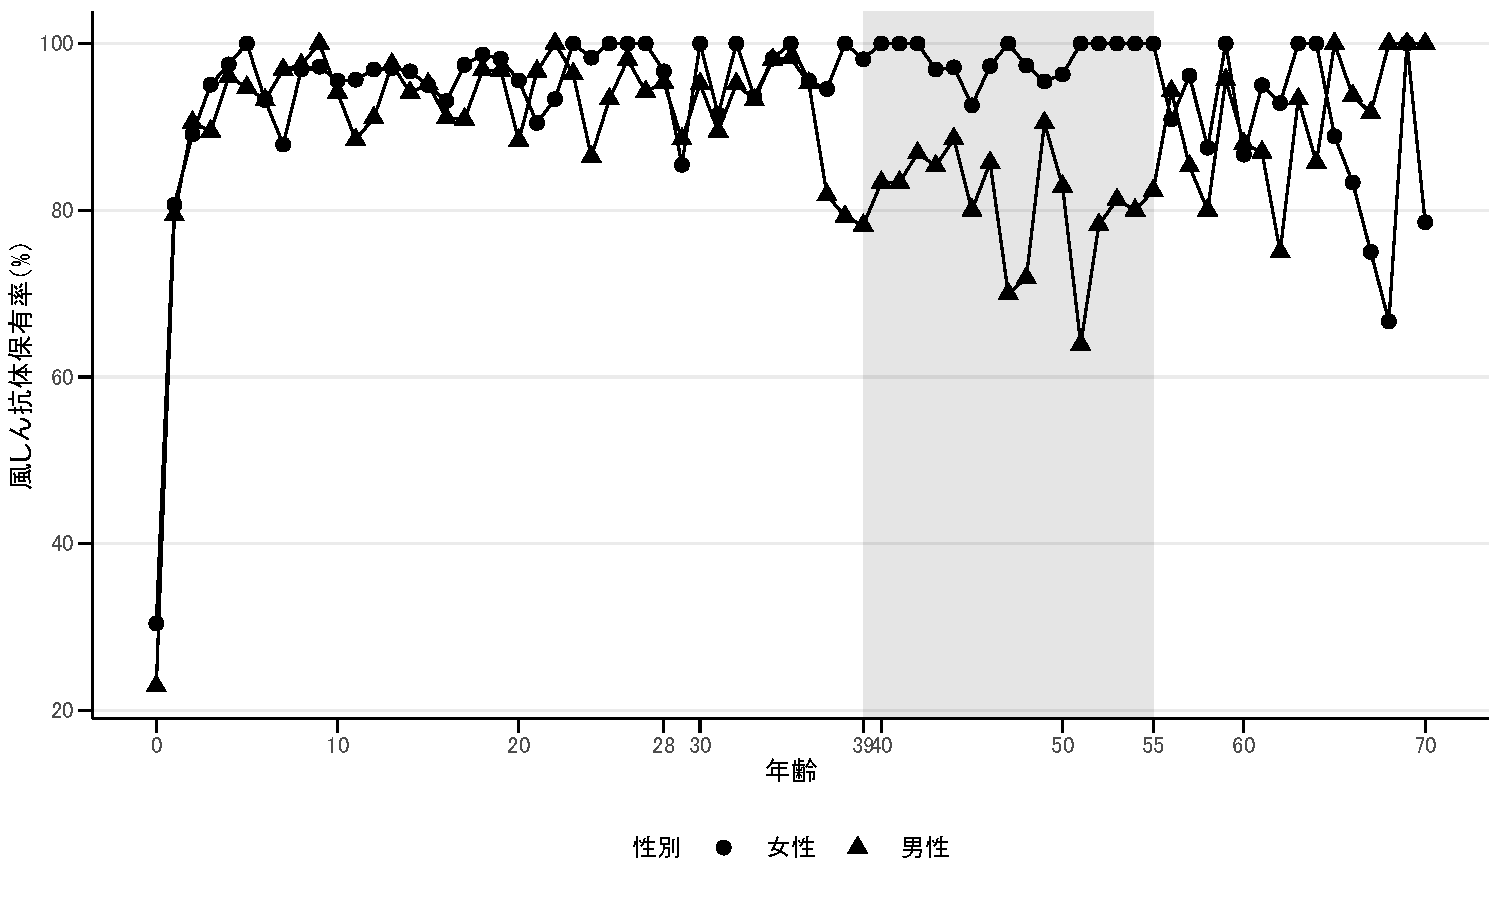
\includegraphics{C:/Users/vge00/Desktop/MHLW-Rubella-Project/2020-online-RCT/publish/body_files/figure-latex/show-niid-antibody-1} \caption{男女別の各年齢における風しん抗体保有率。データソース: 国立感染症研究所『2018年度感染症流行予測調査(NESVPD)』}\label{fig:show-niid-antibody}
\end{figure}

風しんの抗体はワクチン接種だけでなく、自然感染でも得られる。
高齢者を中心に、風しんが流行していた期間に育った人ほど、風しんに自然感染した比率が高くなるので、
風しんワクチンを接種していなくても抗体を保有している可能性が高くなる。
図\ref{fig:show-niid-antibody}は国立感染症研究所(NIID)の
2018年度感染症流行予測調査の男女別・年齢別の風しん抗体保有率をプロットしたものである。
56歳以上の各年齢の抗体保有率の平均は、男女とも約90\%である
(男性:91.3\%、
女性:89.4\%)。
一方、39歳以上55歳以下の(1962年4月2日から1979年4月1日生まれ)の抗体保有率の平均は、
男性では、80.7\%、
女性では、98.3\%である。
つまり、この年齢層の男性の抗体保有率は同世代の女性の抗体保有率より低い。
これは39歳以上55歳以下の男性は風しんワクチンの定期接種の対象外である一方、
39歳以上55歳以下の女性は中学生のときに風しんワクチンを接種していることを反映している。
また、39歳以上55歳以下の男性の抗体保有率は56歳以上の男性のそれよりも低い。
これは56歳以上の男性は、風しんの流行時期に育ったために風しんに自然感染する確率が高かったことを反映している\footnote{このデータを用いて、3つの年齢層(38歳以下・39歳以上55歳以下・56歳以上)と
  女性ダミーの飽和モデルによって抗体保有率を予測した。
  その結果、39歳以上55歳以下の抗体保有率の男女差は
  0.176 (std.error = 0.034; p = 0.000)
  である。また、39歳以上55歳以下の男性と56歳以上の男性の抗体保有率の差は
  0.106 (std.error = 0.036; p = 0.003)
  である。}。

この現状を踏まえて、
厚生労働省は風しんの集団免疫を獲得するために、
2019年4月から2022年3月までの間で、風しん定期接種の追加対策を実施することを決めた。
対象者は抗体保有率が低い1962年4月2日から1979年4月1日生まれの男性(2019年4月時点で40歳から57歳の男性)である。
ワクチン接種の効率的な活用のために、対象の男性は、はじめに抗体検査を受検する。
抗体検査により抗体が持っていないことが明らかになった男性は風しんワクチンを接種する。
この追加対策の目標は、2022年3月までに、対象世代の男性の抗体保有率を90\%に引き上げることである\footnote{妊婦の感染を防ぐという点では、女性の抗体保有率を100\%にするべきという議論も考えられる。
  しかしながら、接種後年数の経過とともに免疫が弱まる可能性や
  1回のワクチン接種だけでは免疫を獲得できない人(約5\%)がいるため、女性の抗体保有率を100\%にすることは難しい。
  したがって、40歳から57歳の男性の抗体保有率を90\%に引き上げて、風しんの集団免疫を獲得するべきである。}。
この目標が達成されれば、すべての世代で抗体保有率が90\%を超え、日本で集団免疫が獲得できる(Kinoshita and Nishiura, 2016)\footnote{Plans-Rubió (2012) によれば、風しんの集団免疫は83\%から95\%の抗体保有率で達成できる。
  Nishiura et al. (2015) では集団免疫が必要な風しんの抗体保有率は83.6\%とされている。}。

この追加対策は予防接種法に基づく定期接種であり、対象となる男性は対象期間において無料で抗体検査とワクチン接種を受けられる。
地方自治体が風しんの抗体検査とワクチン接種の無料クーポン券を3年かけて段階的に対象世代の男性に送付した。
2019年度は、1972年4月2日から1979年4月1日生まれ(2019年4月時点で40-46歳)の男性に市区町村からクーポン券が送付された。
2019年度クーポン券自動送付対象者は約646万人で、追加対策の対象男性の半数以上を占める。
1962年4月2日から1972年4月1日に生まれた男性(2019年4月時点で47-57歳)は2020年度以降にクーポン券を自動的に受け取るが、
市区町村の判断もしくは対象者の希望によって2019年度にクーポン券を受け取ることができた。
2019年1月時点でクーポン券を利用した抗体検査の受検率は約18\%であった\footnote{2019年4月から2020年3月までに40歳から46歳の男性(約646万人)にクーポン券が発送された。
  厚生労働省の聞き取り調査によると、
  2019年10月までに約96\%の自治体がクーポン券の発送を完了する予定であった。
  2019年1月までのクーポン券を利用した抗体検査の累積実績件数は117万件であった。
  抗体検査の受検率は2019年1月までのクーポン券を利用した抗体検査の累積実績件数(117万件)
  を2019年度のクーポン券の発送対象年齢層の40歳から46歳の男性の人口(646万人)で割った値である。
}。

\hypertarget{experiment}{%
\section{オンライン調査の概要}\label{experiment}}

我々はインターネット調査会社であるマイボイスコム株式会社に委託して、合計2回のオンライン調査を実施した。
補論\ref{addtab}の図\ref{fig:show-flowchart}に調査の流れを示した。
第1回調査は2020年2月15日から2020年2月17日に実施した。
第1回調査の対象は調査会社のモニターのうち、日本全国に居住する40歳から59歳の男性の4,200名である。
第1回調査の目的はナッジ・メッセージをランダムに割り当て、
それが風しんの予防行動の意思にどのような影響を与えるかを検証することである。
第2回調査は2020年3月17日から2020年3月25日に実施した。
第2回調査は第1回調査の回答者全員を対象として、3,963名から回答を得た(脱落率=5.64\%)\footnote{脱落率はナッジ・メッセージの群間で統計的に有意な差はない。
  第2回調査に参加しなかったら1を取るダミー変数を被説明変数にし、
  介入群ダミーを説明変数とした線形回帰分析を行った。
  その結果、
  F-value = 1.434 (p-value = 0.197)
  となった。}。
第2回調査の目的は第1回調査でランダムに割り当てたナッジ・メッセージが
実際の予防行動にどのような影響を与えるかを検証することである。

\hypertarget{wave1}{%
\subsection{第1回調査}\label{wave1}}

第1回調査の調査は二つのパートに分けられている(便宜上、質問票Aと質問票Bとする)。
ナッジ・メッセージを示される前に、回答者は質問票Aの質問に回答する。
質問票Aは普段の健康行動などを調査した。
これらの回答の一部を共変量として用いる。
補論\ref{addtab}の表\ref{tab:show-covlist}に共変量の一覧を示す。
また、質問票Aは第1回調査時点で風しんの抗体検査やワクチン接種を受けたかどうかを調査した。
これらの回答はナッジ・メッセージの効果を抗体検査とワクチン接種を受けていない男性に
サンプルを限定して推定するときに使用する。

\begin{table}

\caption{\label{tab:show-nudgelist}ナッジ・メッセージの一覧}
\centering
\fontsize{9}{11}\selectfont
\begin{tabular}[t]{l>{\raggedright\arraybackslash}p{20em}cccccc}
\toprule
\multicolumn{3}{c}{ } & \multicolumn{4}{c}{年齢(2019年4月時点)} & \multicolumn{1}{c}{ } \\
\cmidrule(l{3pt}r{3pt}){4-7}
ナッジ & メッセージ文 &   & 39 & 40-46 & 47-56 & 57-59 & All\\
\midrule
A & 昭和37年度~昭和53年度生まれの男性の皆様へ あなたと、これから生まれてくる世代の子供を守るために風しんの抗体検査と予防接種を受けましょう! & N & 20 & 210 & 321 & 49 & 600\\
B & 40代・50代の男性の皆様へ(昭和37年度~昭和53年度生まれの男性の皆様へ)あなたと、これから生まれてくる世代の子供を守るために風しんの抗体検査と予防接種を受けましょう! & N & 23 & 205 & 309 & 63 & 600\\
C & 40代・50代の男性の皆様へ(昭和37年度~昭和54年度生まれの男性の皆様へ)あなたがきっかけで、妊婦さんが風しんウイルスに感染すると、障害をもった赤ちゃんが産まれてくる可能性があります! & N & 24 & 214 & 296 & 66 & 600\\
D & 40代・50代の男性の皆様へ(昭和37年度~昭和55年度生まれの男性の皆様へ)成人男性が風しんに感染すると、重症化して、脳炎や血小板減少性紫斑病などの合併症が発症する可能性があります! & N & 16 & 225 & 302 & 57 & 600\\
E & 40代・50代の男性の皆様へ(昭和37年度~昭和56年度生まれの男性の皆様へ)あなたの世代の5人に1人は、風しんの抗体を持っていません。これは、他の世代に比べて倍以上の人が風しんに感染する可能性があるということです! & N & 18 & 204 & 321 & 57 & 600\\
F & 40代・50代の男性の皆様へ(昭和37年度~昭和57年度生まれの男性の皆様へ)お届けした風しんの抗体検査とワクチン接種の無料クーポン券は2020年3月31日で有効期限が切れてしまいます! & N & 18 & 216 & 299 & 67 & 600\\
G & 40代・50代の男性の皆様へ(昭和37年度~昭和58年度生まれの男性の皆様へ)風しんの抗体検査とワクチンの無料クーポン券をふだんの健康診断で使えば、何度も採血をすることなく、検査を受けることができます! & N & 19 & 213 & 307 & 61 & 600\\
\bottomrule
\end{tabular}
\end{table}

質問票Aの回答終了後、回答者は7つのメッセージのうち一つをランダムに受け取る。
サンプルサイズが均等になるように、メッセージを年齢層別にランダムに割り当てた\footnote{調査会社が保有する年齢情報を用いて、40~44歳・45~49歳・50~54歳・55~59歳の層別にランダムに割り当てた。各層は1,050名で構成されていて、我々はナッジ・メッセージを均等に割り当てた(150名)。}。
各メッセージのサンプルサイズは600人である。
表\ref{tab:show-nudgelist}はメッセージの一覧とサンプルサイズを示している。
表\ref{tab:show-nudgelist}に示した年齢は調査によって得られた誕生年と誕生月を用いて、2019年4月時点の年齢を計算した\footnote{4月生まれの人はまだ誕生日を迎えていないことを仮定している。また、2019年4月時点での年齢であるため、調査時点で40歳の男性の一部が39歳である。}。
2019年4月時点で40歳から56歳の男性が厚労省の追加的対策の対象であり、
40歳から46歳の男性は1年目にクーポン券を自動的に受け取る。

ナッジ・メッセージは厚生労働省のホームページにあるメッセージ
「昭和37年度~昭和53年度生まれの男性の皆様へ 
あなたと、これから生まれてくる世代の子どもを守るために風しんの抗体検査と予防接種を受けましょう!」
に基づいており、厚労省メッセージと呼ぶ。

各ナッジ・メッセージには、厚労省メッセージを(1)簡易な年齢表現と(2)行動経済学に基づいたメッセージ内容に変更したものを用意した。
年齢表現メッセージは風しんの追加対策の正確な対象年齢に加えて、「40代・50代の男性」という平易な表現を追加した。
これは自分が接種対象者であるかどうかが容易に理解できるようにして、メッセージ自体の注意を引くことを目的としている。
年齢表現メッセージは年齢表現を変えただけで、メッセージの内容は原文と同じであるが、
それ以外のナッジ・メッセージは年齢表現だけでなく、行動経済学の知見に基づいたメッセージ内容に変更した。

利他強調メッセージは自身が感染することで他人(特に、妊婦)にどのような損害を与えるかを具体的に記述している。
これは負の外部性を容易に想起させ、外部性を考慮する利他的な人の行動変容を促すことを目的としている。

利己強調メッセージ・社会比較メッセージは風しんの抗体を持つことの価値を高めることで行動変容を促すという目的で作成された。
利己強調メッセージは自身が感染することで自分がどのような損害を受けるかを具体的に記述し、
自身が感染することで生じる自身の損害を容易に想像できるようにした。
社会比較メッセージは抗体保有率が低いことを明記して、自身が感染しやすいことを強調している。
これは風しんの感染確率を過小に見積もることを通じてワクチン接種の価値を過小に評価することを防ぐことができる。

有効期限メッセージと低コストメッセージは風しんのクーポン券制度に関する内容に変更した。
有効期限メッセージはクーポンの有効期限を強調する内容である。
2019年度に配布されるクーポン券には、2020年3月31日が有効期限であることを明記していた。
このメッセージは再度その内容を明記した。
これは現在バイアスによって抗体検査の受験やワクチン接種が妨げられていることを防ぐ目的で作成した。
低コストメッセージは健康診断のついでに抗体検査を受診できることを明記して、簡単に受検できることを強調する内容である。
このメッセージは抗体検査の主観的なコストを抑える目的で作成した。

ランダムに割り当てられたナッジ・メッセージを閲覧した後、回答者は質問票Bに移る。
質問票Bは抗体検査の受検やワクチン接種に関する意思を調査した\footnote{質問票Bでは、教育年数や婚姻状態などの個人の社会経済変数についても調査している。
  これらの変数は共変量として用いる(補論\ref{addtab}の表 \ref{tab:show-covlist})。}。
ナッジ・メッセージの意向に対する効果を推定するとき、この回答をアウトカム変数として用いる。
抗体検査受検の意向は「今、あなたは、風しんの抗体検査を受けようとどのくらい思っていますか」という質問である。
ワクチン接種の意向は「抗体検査を受けて、あなたに抗体がないと分かった場合、
あなたは、ワクチンを接種しようとどのくらい思いますか」という質問である。
それぞれの質問に対して、
回答者は「絶対に受ける」「受ける」「どちらともいえない」「受けない」「絶対に受けない」「すでに受けた」で回答する。
我々は「絶対に受ける」もしくは「受ける」と回答したら1を取るダミー変数をアウトカム変数として用いる。

\hypertarget{wave2}{%
\subsection{第2回調査}\label{wave2}}

第2回調査は第1回調査以降に抗体検査の受検やワクチン接種したかどうかを調査した\footnote{第2回調査の調査時期は新型コロナウイルスの流行が始まった時期と重なるので、
  それが健康行動などに大きな変化を与えた可能性がある。
  この可能性をコントロールするために、日常の詳細な健康行動についても調査した。
  その回答は共変量として用いる(補論\ref{addtab}の表 \ref{tab:show-covlist})。}。
抗体検査の受検行動は
「前回のアンケートの回答終了時から今日までの期間に、あなたは風しんの抗体検査を受診しましたか」
という質問で得られる。
回答者は「受診した」・「受診していない」・「前回アンケートより以前に、受診済みである」から一つ選ぶ。
ワクチン接種行動は
「前回のアンケートの回答終了時から今日までの期間に、あなたは風しんワクチンを接種しましたか」
という質問で得られる。
回答者は「接種した」・
「すでに抗体検査で十分に抗体があることを確認した・すでに風しんに感染したので、接種する必要がなかった」・
「すでに抗体検査で十分に抗体がないことを確認したが、まだ接種していない」・
「抗体検査の受診もワクチンの接種もしていない」・
「前回アンケートより以前に、接種済みである」
から一つ選ぶ。

これらの回答を用いて、二つのアウトカム変数を作成する。
第一のアウトカム変数は回答者が「受検した」と回答すると1を取るダミー変数である。
このアウトカム変数を用いて、我々は第1回調査以降の抗体検査の受検に対するナッジ・メッセージの効果を推定する。
第二のアウトカム変数は回答者が抗体検査を「受検した」と回答し、
ワクチンを「接種した」と回答すると1を取るダミー変数である。
厚生労働省の政策目標は抗体を持っていない人がワクチン接種を受けることで抗体保有率を引き上げることである。
したがって、このアウトカム変数は政策目標に直結している。

\hypertarget{result}{%
\section{分析結果}\label{result}}

\hypertarget{selection}{%
\subsection{サンプルセレクションの定義}\label{selection}}

我々の関心はナッジ・メッセージが抗体検査やワクチン接種を受けていない男性の行動を促進できるかどうかである。
そのために、第1回調査時点で抗体検査とワクチン接種を受けていない男性にサンプルを限定して、
ナッジ・メッセージの効果を推定する。
分析に用いるサンプルの基準は2つある。
第一の基準は第1回調査で過去に抗体検査を受検したもしくは過去にワクチン接種をしていないと回答したかどうかである。
抗体検査の受検やワクチン接種の意向に対する効果を推定するとき、
この基準を満たした男性にサンプルを限定する(以降、Wave 1セレクションデータと呼ぶ)。
第二の基準は第2回調査で第1回調査以前に抗体検査を受検したもしくはワクチンを接種したと回答したかどうかである\footnote{第1回調査以降に自身の接種歴を調べ直すなどによって、第1回調査と第2回調査の回答に違いが生じる可能性がある。
  そのため、どちらかの調査で第1回調査以前に抗体検査を受検したもしくはワクチンを接種したと回答した人を除いた。}。
第1回調査以降の抗体検査の受検やワクチン接種に対する効果を推定するとき、
第一の基準と第二の基準を満たした男性にサンプルを限定する(以降、Wave 2セレクションデータと呼ぶ)。

我々は上記の基準で構築したサブサンプルを2019年度にクーポン券の送付対象年齢か否かで分割して、
各グループにおけるナッジ・メッセージの効果を推定する。
2019年度にクーポン券の送付対象年齢か否かは2019年4月時点の年齢で識別した。
各市区町村は2019年度に40歳以上46歳以下の男性のクーポン券を送付し、
2020年度以降に47歳以上56歳以下の男性のクーポン券を送付する。
ただし、市区町村の判断や本人の希望に応じて、47歳以上56歳以下の男性もクーポン券を受け取ることはできる。

\hypertarget{coupon1}{%
\subsection{2019年度クーポン券配布対象者に限定したナッジ・メッセージの効果}\label{coupon1}}

始めに、2019年度にクーポン券が送付された40歳以上46歳以下の男性グループにおける、
ナッジ・メッセージの意向と行動に対する効果を推定する。
このサブグループにおいて、回答者の観察可能な特徴についてトリートメント間でバランスしている
(補論\ref{addtab}の表\ref{tab:show-int-coupon1-balance}
と表\ref{tab:show-act-coupon1-balance})。
したがって、本節では、
厚労省メッセージと各ナッジ・メッセージ間の平均値の差の検定の結果のみを示し、
回帰分析の結果は補論に示す。
また、検出力80\%・有意水準5\%を保つために必要な効果の規模を計算したところ、
意向をアウトカムとした場合は少なくとも
6.7
\%ポイント必要であり、
行動をアウトカムとした場合は少なくとも
7.2
\%ポイント必要である。

\begin{figure}[t]
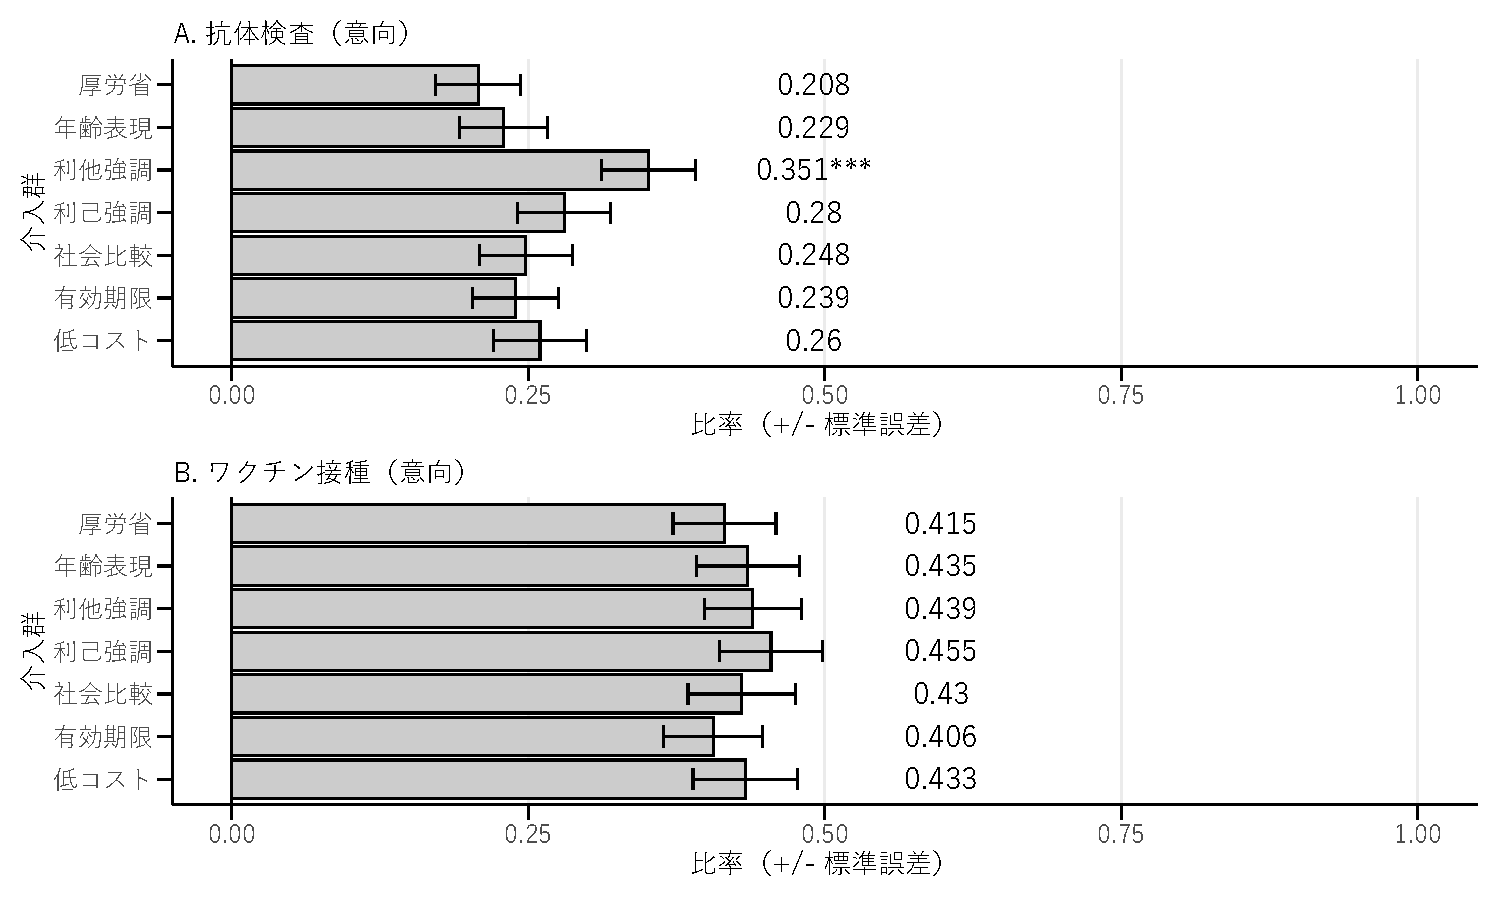
\includegraphics{C:/Users/vge00/Desktop/MHLW-Rubella-Project/2020-online-RCT/publish/body_files/figure-latex/show-int-coupon1-ttest-1} \caption{2019年度クーポン券配布対象者に限定した意向に対するナッジ・メッセージの効果。データソース:Wave 1セレクションデータ。注)図中の数値は各群の比率を示す。星印は厚労省メッセージ群との平均値の差のt検定の結果であり、次の規則に従う:* p < 0.1、** p < 0.05、*** p < 0.01。}\label{fig:show-int-coupon1-ttest}
\end{figure}

図\ref{fig:show-int-coupon1-ttest}のパネルAは
各介入群の抗体検査受検の意向を示している。
結果として、
利他強調メッセージは厚労省メッセージよりも抗体検査受検の意向を高めている。
厚労省メッセージを読んだ人の約20.8\%が抗体検査を受けたいと回答している一方で、
利他強調メッセージを読んだ人の約35.1\%が抗体検査を受けたいと回答している。
したがって、
利他強調メッセージはコントロールよりも
約14.3\%ポイント抗体検査の受検意向を引き上げており、
これはt検定より統計的に1\%水準で有意である。
その他のナッジ・メッセージについては、
抗体検査を受けたいと答えた人の割合は30\%を下回っていて、
その比率が厚労省メッセージと等しいという帰無仮説を棄却できない。

図\ref{fig:show-int-coupon1-ttest}のパネルBは
各介入群のワクチン接種の意向を示している。
その結果、すべてのナッジ・メッセージ群における比率は40\%から45\%の範囲にあり、
それが厚労省メッセージの比率と統計的に有意な差とならなかった。
考えられる可能性の一つはワクチン接種の意向の質問文による刺激である。
我々は抗体を持っていないという条件のもとで接種したいかどうかを質問しているので、
質問文がワクチン接種の必要性を強く刺激した可能性がある。

\begin{figure}[t]
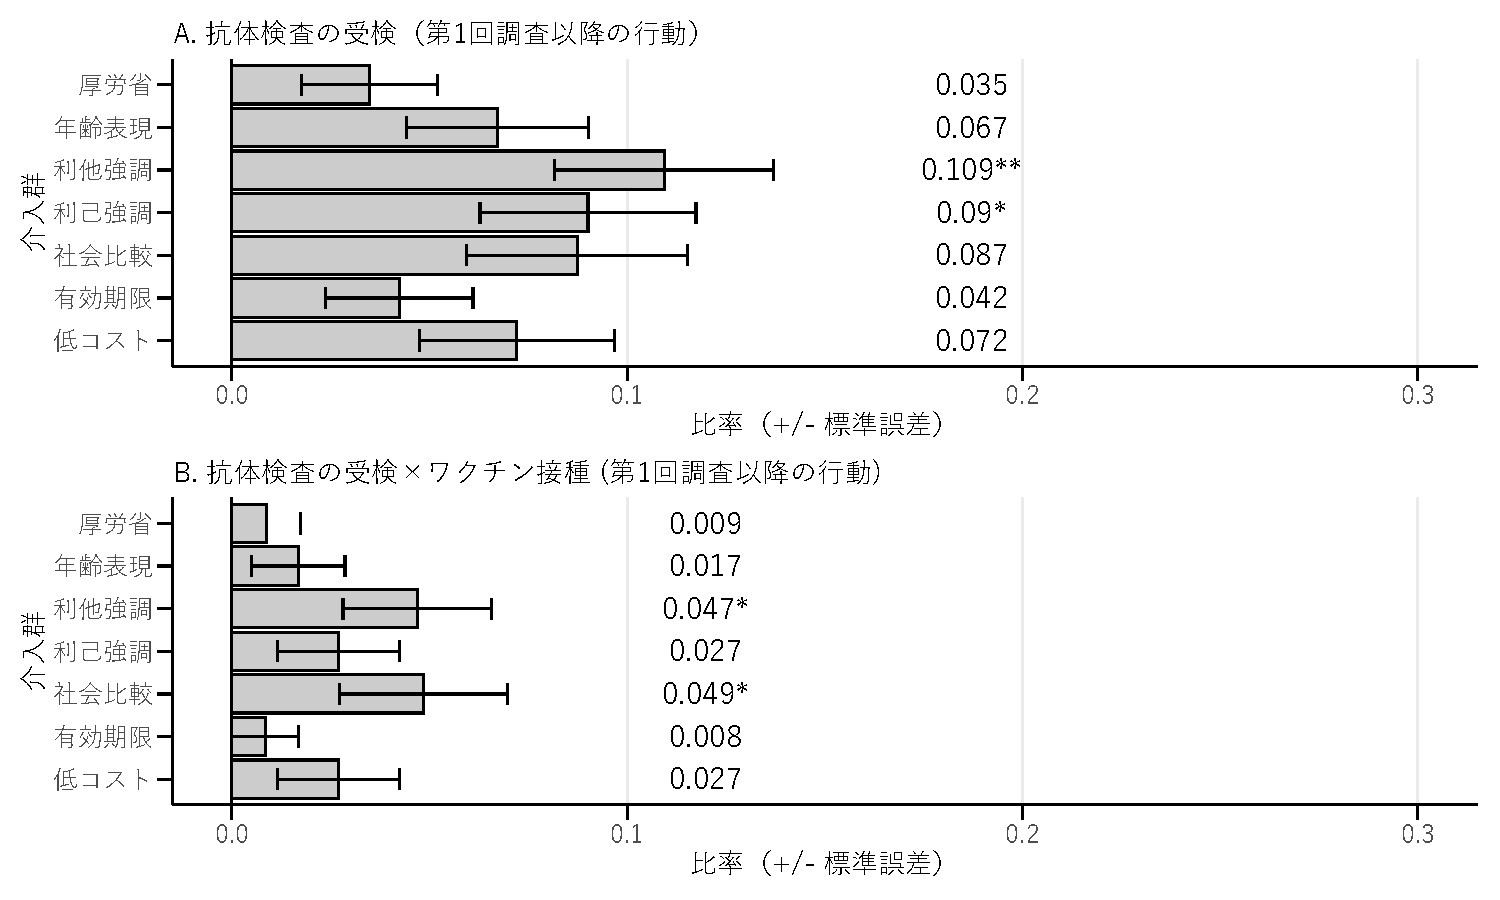
\includegraphics{C:/Users/vge00/Desktop/MHLW-Rubella-Project/2020-online-RCT/publish/body_files/figure-latex/show-act-coupon1-ttest-1} \caption{2019年度クーポン券配布対象者に限定した行動に対するナッジ・メッセージの効果。データソース:Wave 2セレクションデータ。注)図中の数値は各群の比率を示す。星印は厚労省メッセージ群との平均値の差のt検定の結果であり、次の規則に従う:* p < 0.1、** p < 0.05、*** p < 0.01。}\label{fig:show-act-coupon1-ttest}
\end{figure}

図\ref{fig:show-act-coupon1-ttest}のパネルAは各介入群の第1回調査以降の抗体検査受検比率を示している。
結果として、利他強調メッセージと利己強調メッセージでは、厚労省メッセージよりも
第1回調査以降の抗体検査の受検比率が高い。
厚労省メッセージを読んだ人の約3.5\%は第1回調査以降に抗体検査を受検している。
その一方で、利他強調メッセージを読んだ人の約10.9\%と
利己強調メッセージを読んだ人の約9\%は第1回調査以降に抗体検査を受検している。
したがって、利他強調メッセージはコントロールに比べて7.4\%ポイント抗体検査の受検率を引き上げており、
これはt検定より統計的に5\%水準で有意である。
また、利己強調メッセージはコントロールよりも約5.5\%ポイント高く、これはt検定より統計的に10\%水準で有意である。

図\ref{fig:show-act-coupon1-ttest}のパネルBは
各介入群の第1回調査以降の抗体検査とワクチン接種を両方受けた人の比率(以降、ワクチン接種率と呼ぶ)を示している。
この比率は今回の厚生労働省の政策によって新たに抗体を獲得した人の比率を示すので、
政策効果のアウトカム指標となる。
その結果、利他強調メッセージと社会比較メッセージがワクチン接種を促進していることがわかる。
厚労省メッセージを読んだ人の約0.9\%が抗体検査を受検し、ワクチンを接種している。
その一方で、利他強調メッセージを読んだ人の約4.7\%と
社会比較メッセージを読んだ人の約4.9\%が第1回調査以降に抗体検査を受検し、ワクチンを接種している。
よって、利他強調メッセージは3.8\%ポイントコントロールよりも高く、これはt検定より統計的に10\%水準で有意である。
社会比較メッセージは4\%ポイントコントロールよりも高く、これはt検定より統計的に10\%水準で有意である。

補論\ref{addtab}の表\ref{tab:show-int-coupon1-reg}
と表\ref{tab:show-act-coupon1-reg}に厚労省メッセージ群を比較対象とした
ナッジ・メッセージの線形確率モデルの推定結果を示した。
ここまでの結果は個人の観察可能な特徴をコントロールしても変化しない。
それに加えて、共変量を制御したモデルを推定すると、
利己強調メッセージは厚労省メッセージよりも抗体検査受検の意向を約9\%ポイント強めていて、
これは統計的に10\%水準で有意である。
さらに、利己強調メッセージと社会比較メッセージは厚労省メッセージと比較して抗体検査の受検行動に
統計的に5\%水準で正の影響を与えている。
効果の規模はそれぞれ6.7\%ポイントと6.5\%ポイントである。

また、効果の規模が最も大きい利他強調メッセージ群を比較対象とした
線形確率モデルの推定結果を補論\ref{addtab}の
表\ref{tab:show-int-coupon1-altreg}と
表\ref{tab:show-act-coupon1-altreg}に示した。
その結果、
利己強調メッセージ群の抗体検査受検の意向は利他強調メッセージのそれと統計的に有意な差とならなかった。
さらに、利己強調メッセージと社会比較メッセージの抗体検査の受検比率は
利他強調メッセージのそれと統計的に有意に異ならならなかった。
したがって、効果があった利他強調メッセージとの有意差がないという意味で、
利己強調メッセージは抗体検査受検の意向と行動を促進した可能性があり、
社会比較メッセージは抗体検査の受検を促進した可能性がある。
しかしながら、抗体検査の受検比率の差は検出力を十分に保つほどの大きさではないので、
サンプルサイズを十分に大きくして検証する必要がある。

\begin{table}

\caption{\label{tab:show-tester-coupon1}2019年度クーポン券配布対象の抗体検査受検者の動き}
\centering
\begin{threeparttable}
\begin{tabular}[t]{lcccc}
\toprule
\multicolumn{1}{c}{ } & \multicolumn{2}{c}{Negative antibody} & \multicolumn{2}{c}{Vaccination} \\
\cmidrule(l{3pt}r{3pt}){2-3} \cmidrule(l{3pt}r{3pt}){4-5}
Treatments & No & Yes & No  & Yes \\
\midrule
厚労省 & 3 & 1 & 3 & 1\\
年齢表現 & 6 & 2 & 6 & 2\\
利他強調 & 7 & 7 & 8 & 6\\
利己強調 & 7 & 3 & 7 & 3\\
社会比較 & 4 & 5 & 4 & 5\\
有効期限 & 4 & 1 & 4 & 1\\
低コスト & 3 & 5 & 5 & 3\\
\bottomrule
\end{tabular}
\begin{tablenotes}
\item Note: Fisher exact test (Outcome: Negative antibody): p = 0.543. Fisher exact test (Outcome: Vaccination): p = 0.85.
\end{tablenotes}
\end{threeparttable}
\end{table}

我々のサーベイには抗体検査の結果の情報があるので、
その変数を用いて先の結果に関するメカニズムを議論しよう。
そのために、我々は抗体検査を受検した人に限定して、
抗体検査の結果とトリートメント群のクロス集計と、
ワクチン接種とトリートメント群のクロス集計を作成し、
それを表\ref{tab:show-tester-coupon1}に示した。

この表から二つの発見がある。
第一に、各群の陰性者のワクチン接種率は60\%から100\%の範囲にある。
たとえば、利他強調メッセージを割り当てられた抗体検査受検者は14人いるが、
そのうち7人が抗体を保有していなかった。
さらに、制度上、陰性者のみがワクチンを接種するので、
抗体を保有していない7人のうち6人がワクチンを接種している。
よって、陰性者のワクチン接種率は85.7\%(\(=6/7\))である。
また、サンプルをトリートメント群で分割しない場合、陰性者のワクチン接種率は87.5\%であり、
その95\%信頼区間は100\%を含んでいる\footnote{1000個のブートストラップ標本を用いて、陰性者のワクチン接種率の95\%信頼区間を計算すると、
  {[}75.0\%, 100.0\%{]}
  となった。}。
したがって、介入に関わらず抗体検査の結果が陰性である人のほとんどがワクチンを接種している。

第二に、各群の抗体検査の陰性比率は20\%から62.5\%の範囲にある。
たとえば、利他強調メッセージを割り当てられた抗体検査受検者14人のうち、
7人が抗体を保有していなかったので、陰性比率は50\%である。
また、厚労省メッセージ群と社会比較メッセージ群における陰性比率はそれぞれ
25\%(\(=1/4\))と55\%(\(=5/9\))である。
したがって、利他強調メッセージと社会比較メッセージは
厚労省メッセージよりも抗体検査の受検を促進しただけでなく、
ワクチンを接種する必要のある受検者が多くいたので、ワクチン接種に対して正の効果があった。
逆に、利己強調メッセージの陰性比率は30\%(\(=3/10\))であり、
厚労省メッセージ群のそれと近い値になったので、
抗体検査の受検に対して正の効果があるにも関わらず、
ワクチン接種に対して統計的に有意でなかった。
ただし、群間で陰性比率が大きく異なるという結果は母集団では当てはまらない可能性が高い\footnote{これと対立する仮説として、
  利他強調メッセージや社会比較メッセージを読んで抗体検査を受検した人は
  自身に抗体を保有していないと信じているということが考えられる。
  そこで、陰性者の抗体検査受検率を推定することを試みる。
  しかしながら、陰性であるにも関わらず抗体検査を受検していない人がいるはずなので、
  陰性者の抗体検査受検率をデータから直接復元することはできない。
  我々は、ベイズ定理を用いて、間接的に推定した。
  陰性という事象\(A\)と抗体検査の受検という事象\(B\)の二つの事象を考える。
  このとき、抗体検査の受検比率は\(P(B)\)、抗体検査受検者の陰性比率は\(P(A|B)\)で表すことができ、
  これらの値はデータから直接推定できる。
  ベイズの定理より、抗体検査受検者の陰性比率は
  \[ P(A|B) = \frac{P(B|A) \cdot P(A)}{P(B)} \]
  と定義できる。
  ここで、\(P(A)\)は陰性比率であり、
  これは第\ref{background}節で示したNIIDのデータより0.2となる。
  確率\(P(B|A)\)は陰性者で条件づけた抗体検査の受検比率であり、我々の関心のあるパラメータである。
  よって、陰性者の抗体検査の受検比率は
  \[ \hat{P}(B|A) = \frac{\hat{P}(A|B) \cdot \hat{P}(B)}{0.2} \]
  で計算できる。
  利他強調メッセージ群において、
  \(\hat{P}(A|B) = 0.5\)と\(\hat{P}(B) = 0.109\)なので、
  \(\hat{P}(B|A) = 0.273\)となる(1000個のブートストラップ標本で構築した95\%信頼区間は
  {[}0.117, 0.469{]}
  さらに、陰性であるかどうかによって抗体検査の受検にセレクションが生じているかどうかを
  検証するために、陰性という事象と抗体検査の受検という事象が独立であるという帰無仮説を検定した。
  \(\hat{P}(B|A) - \hat{P}(B)\)の95\%信頼区間にゼロが含まれていないとき、
  我々は帰無仮説を5\%有意水準で棄却できる。
  その結果、\(\hat{P}(B|A) - \hat{P}(B)\)の95\%信頼区間は
  {[}0.016, 0.336{]}
  なので、我々は帰無仮説を棄却できる。
  同様に、社会比較メッセージ群の\(\hat{P}(B|A) - \hat{P}(B)\)の95\%信頼区間は
  {[}0.000, 0.350{]}
  である。
  したがって、利他強調メッセージ群と社会比較メッセージ群では、
  陰性者が抗体検査を積極的に受検している傾向があるかもしれない。}。
ナッジ・メッセージの割り当てと陰性という事象が独立であるという帰無仮説を
フィッシャーの正確検定で検証したところ、
我々はその帰無仮説を棄却できなかった(p値=0.543)。

\hypertarget{econvalue}{%
\subsection{ナッジ・メッセージの金銭的価値}\label{econvalue}}

\begin{figure}[t]
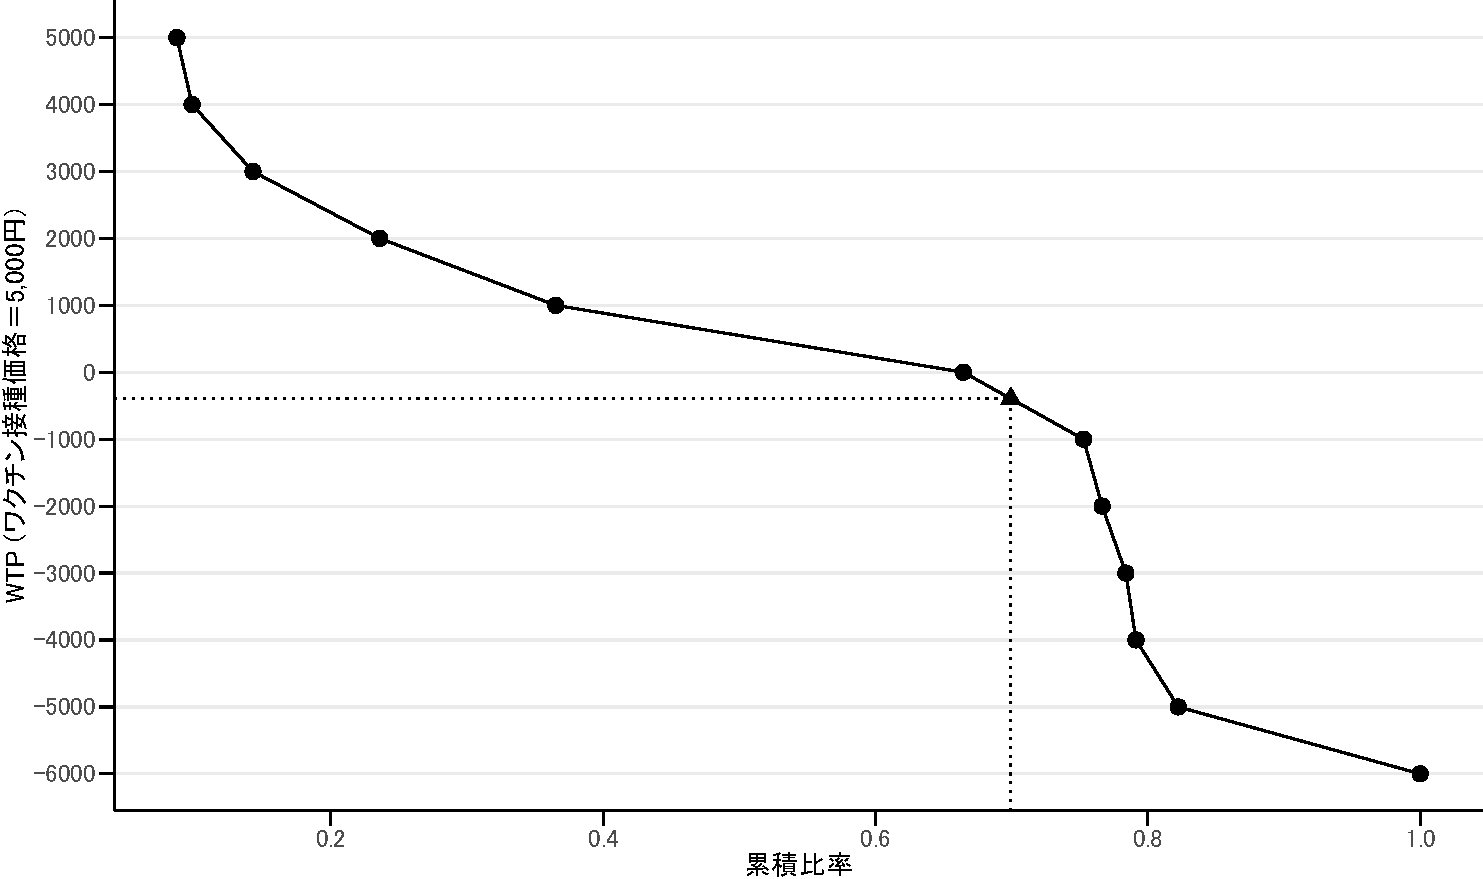
\includegraphics{C:/Users/vge00/Desktop/MHLW-Rubella-Project/2020-online-RCT/publish/body_files/figure-latex/show-demand-vaccine-1} \caption{2019年度クーポン券配布対象者の風しんワクチンの需要曲線。データソース:Wave 1セレクションデータ。注)黒の三角はワクチン接種費用が無料であるときの接種割合と厚労省メッセージの抗体検査受検率を合計した割合と、それに対応するWTPを示している。}\label{fig:show-demand-vaccine}
\end{figure}

2019年度のクーポン券送付者におけるナッジ・メッセージの効果を金銭的な価値で評価することを試みる。
そのために、第1回調査のナッジ・メッセージを示す前の質問票Aで調査したワクチン接種の支払意思額を用いる。
ワクチンの価格は5000円と仮定して、我々は、自治体の補助金額が\(s_j\)のとき、ワクチン接種をするかどうかを調査した。
補助金額は\(s_j \in \{0, 1000, 2000, \ldots, 10000\}\)とした。
回答者\(i\)が接種すると回答した最低の補助金額を\(s_i^{\text{min}}\)とする。
回答者\(i\)が接種しないと回答した最高の補助金額を\(s_i^{\text{max}}\)とする。
このとき、回答者\(i\)の支払意思額は
\([5000 - s_i^{\text{min}}, 5000 - s_i^{\text{max}})\)の範囲内で識別される\footnote{回答者がすべての補助金額\(s_j\)のときの接種しないと回答したならば、\(s_i^{\text{max}} = 10000\)である。しかしながら、\(s_i^{\text{min}}\)はデータで定義できない。そこで、\(s_i^{\text{min}} = 11000\)と仮定した。ただし、後に示すが、この仮定はナッジ・メッセージの金銭的価値に影響を与えない。}。
したがって、追加の仮定を置かない限り、ワクチン接種の需要曲線はステップワイズな曲線となり、
メッセージの金銭的価値は範囲で得られる。

メッセージの金銭的価値を点推定するために、
我々は支払意思額が\([5000 - s_i^{\text{min}}, 5000 - s_i^{\text{max}})\)の範囲で識別されるとき、
真の支払意思額はその範囲内で一様に分布することを仮定する。
このとき、ステップワイズなワクチン接種の需要曲線は線型補間で表される。
図\ref{fig:show-demand-vaccine}はこの仮定のもとで、2019年度に自動的にクーポン券を受け取る人に限定した
風しんワクチン接種の需要曲線である。
我々はこの需要曲線を用いて、メッセージの金銭的価値を算出する。

\begin{table}

\caption{\label{tab:show-economic-value}ナッジ・メッセージの金銭的価値の推定}
\centering
\resizebox{\linewidth}{!}{
\fontsize{9}{11}\selectfont
\begin{threeparttable}
\begin{tabular}[t]{lcccccc}
\toprule
\multicolumn{3}{c}{ } & \multicolumn{2}{c}{金銭的価値(日本円)} & \multicolumn{2}{c}{金銭的価値(米ドル)} \\
\cmidrule(l{3pt}r{3pt}){4-5} \cmidrule(l{3pt}r{3pt}){6-7}
ナッジ・メッセージ & 効果の規模 & ベースライン+効果の規模 & 一人当たり & 総額 & 一人当たり  & 総額 \\
\midrule
年齢表現 & 0.032 & 0.732 & 367.854 & 1.946 & 3.344 & 17.690\\
利他強調 & 0.075 & 0.774 & 2037.553 & 10.779 & 18.523 & 97.988\\
利己強調 & 0.055 & 0.755 & 744.045 & 3.936 & 6.764 & 35.782\\
社会比較 & 0.053 & 0.752 & 596.335 & 3.155 & 5.421 & 28.678\\
有効期限 & 0.008 & 0.707 & 86.059 & 0.455 & 0.782 & 4.139\\
低コスト & 0.037 & 0.737 & 422.789 & 2.237 & 3.844 & 20.332\\
\bottomrule
\end{tabular}
\begin{tablenotes}
\item 注) 抗体検査の受検に対するナッジ・メッセージの効果を効果の規模として用いた。 ベースラインはワクチン接種費用が無料であるときの接種割合と 厚労省メッセージの抗体検査受検率を合計した割合である。 金銭的価値は一人当たりの価値と それに2020年1月時点でワクチンクーポン券を利用していない人数(529万人)をかけた 総額を示している。 また、金銭的価値は日本円と米ドルで示した(1ドル=110円)。 一人当たりの金銭的価値の単位はそれぞれ1円と1ドルである。 総額で示した金銭的価値の単位はそれぞれ10億円と100万ドルである。
\end{tablenotes}
\end{threeparttable}}
\end{table}

ナッジ・メッセージの金銭的な価値を次のように計算する。
はじめに、ベースラインの接種割合を決める。
図\ref{fig:show-demand-vaccine}の需要曲線は無料クーポンが発行される人に限定しているので、
ワクチンの供給曲線はゼロで水平である。
このときの接種割合は約66.5\%である。
ベースラインの接種割合はこの割合に厚労省メッセージの抗体検査受検率を足したものとする\footnote{抗体検査の結果が陰性である人のほとんどはワクチンを接種しているので、
  抗体検査の受検率をワクチン接種率として用いる。}。
ベースラインの接種割合は約70\%であり、対応する支払意思額は約-394円である。

次に、接種割合をベースラインの均衡点からナッジ・メッセージの効果分だけ増やすとき、
需要曲線上で対応する支払意思額を見つける。
その支払意思額はナッジ・メッセージの効果量だけ増やすのに必要な自治体の追加的な補助金額であり、
それがナッジ・メッセージの一人当たりの金銭的価値である。
たとえば、ベースラインの均衡点の接種割合とナッジ・メッセージの効果の和が0.8であるとき、
需要曲線上で対応する支払意思額は約-4280円である。
すなわち、ナッジ・メッセージの効果量分だけ接種割合を増やすために、
自治体は一人当たり約3886(\(=4280-394\))円の追加的な補助金を支払う必要がある。

我々は抗体検査受検に対するナッジ・メッセージの効果を用いる。
表\ref{tab:show-tester-coupon1}で示したように、
抗体検査の結果が陰性である人のほとんどはワクチンを接種している。
したがって、抗体検査受検に対するナッジ・メッセージの効果をワクチン接種に対する効果とみなせる。

表\ref{tab:show-economic-value}はメッセージの金銭的価値の試算結果である。
第2列は図\ref{fig:show-act-coupon1-ttest}のパネルAで示したメッセージの効果を示している。
第3列はベースラインの均衡点の接種割合からメッセージの効果量分だけ増やしたときの接種割合を示している。
第4列はメッセージの一人当たりの金銭的価値である。
この金銭的価値をアメリカドルに換算した結果を第6列に示している。
抗体検査の受検を促進した利他強調メッセージの一人当たりの金銭的価値は約2000円(約18ドル)である。

また、メッセージ自体の金銭的価値の総額は一人当たりの金銭的価値と
2019年度に発行されたクーポン券をまだ利用していない人数の積で得られる。
厚生労働省より、2019年度にクーポン券が発行されたにもかかわらず、
1月時点で抗体検査のクーポン券を利用していない人は約529万人である。
表\ref{tab:show-economic-value}の第5列はメッセージの金銭的価値の総額を示している。
第7列はそれをアメリカドルに換算した結果を示している。
利他強調メッセージの金銭的価値の総額は約100億円である。

\hypertarget{coupon0}{%
\subsection{2019年度クーポン券送付対象外の男性に限定したナッジ・メッセージの効果}\label{coupon0}}

次に、2019年度には、クーポン券の自動送付対象ではないが、
自身が手続きすることでクーポン券を受け取れる人に限定して、
ナッジ・メッセージの効果を推定する。
このサブグループにおいて、
回答者の観察可能な特徴についてトリートメント間でバランスしている
(補論\ref{addtab}の表\ref{tab:show-int-coupon0-balance}
と表\ref{tab:show-act-coupon0-balance})。
よって、\ref{coupon1}と同様に、この節ではt検定の結果のみを示し、回帰分析の結果は補論に示す。
検出力80\%・有意水準5\%を保つために必要な効果の規模を計算したところ、
意向をアウトカムとした場合は少なくとも
5
\%ポイント必要であり、行動をアウトカムとした場合は少なくとも
5.3
\%ポイント必要である。

\begin{figure}[t]
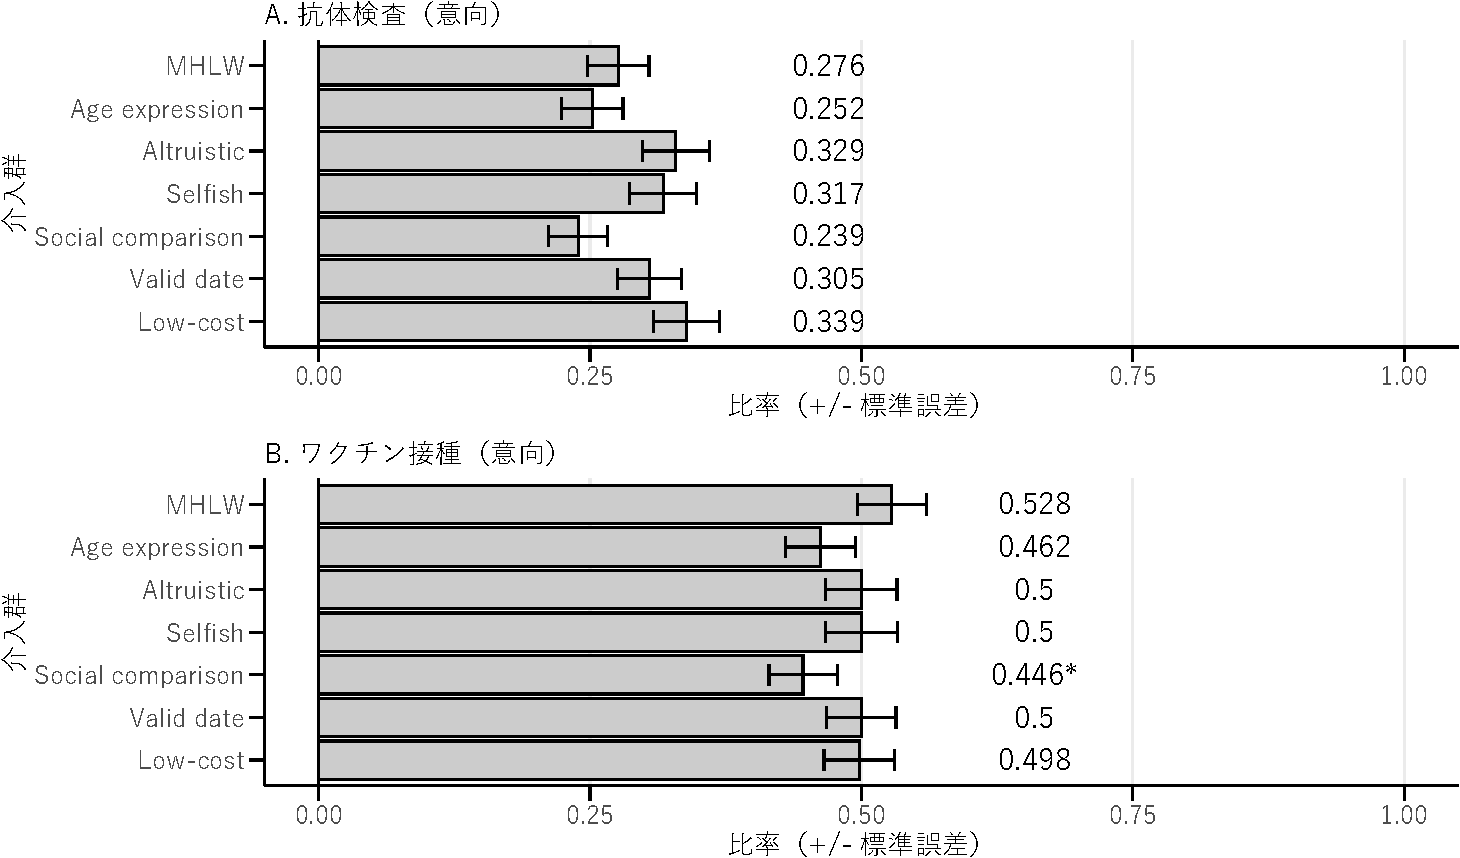
\includegraphics{C:/Users/vge00/Desktop/MHLW-Rubella-Project/2020-online-RCT/publish/body_files/figure-latex/show-int-coupon0-ttest-1} \caption{2019年度クーポン券配布対象外の男性に限定した意向に対するナッジ・メッセージの効果。データソース:Wave 1セレクションデータ。注)図中の数値は各群の比率を示す。星印は厚労省メッセージ群との平均値の差のt検定の結果であり、次の規則に従う:* p < 0.1、** p < 0.05、*** p < 0.01。}\label{fig:show-int-coupon0-ttest}
\end{figure}

図\ref{fig:show-int-coupon0-ttest}は介入群ごとの抗体検査受検とワクチン接種の意向の比率を示している。
図\ref{fig:show-int-coupon1-ttest}と同様に、すべての介入群について、
抗体検査受検の意向の比率はワクチン接種の意向の比率より低い。
2019年度にクーポン券が送付されない人に対しても、
ワクチン接種の意向の質問文は抗体検査が陰性だったという条件付であることに注意して解釈すべきである。

また、社会比較メッセージは抗体検査受検の意向に対して統計的に有意な効果を持っていないが、
ワクチン接種の意向に対して負の効果を持っている。
厚労省メッセージを読んだ人の抗体検査受検とワクチン接種の意向の比率はそれぞれ約27.6\%と約52.8\%である。
それに対して、社会比較メッセージを読んだ人の抗体検査受検とワクチン接種の意向の比率はそれぞれ
約23.9\%と約44.6\%である。
したがって、社会比較メッセージの抗体検査受検の意向に対する効果は約-3.7\%ポイントであり、
これは統計的に有意な効果ではない。
しかしながら、社会比較メッセージのワクチン接種の意向に対する効果は約-8.2\%ポイントであり、
これは統計的に10\%水準で有意である。

この負の効果の原因の一つとして、ワクチン接種のただ乗りが挙げられる。
社会比較メッセージは「5人に1人が抗体を持っていない」ことを強調している。
裏返せば、5人に4人が抗体を持っているということである。
このメッセージを読んだ人は、仮に風しんの抗体を保有していないとしても、
全体の80\%が抗体を持っているので、自身が感染する機会は少ないと考えたのかもしれない。
クーポン券がない場合、
この信念がワクチンを接種することの価値を低め、
ワクチン接種の意向の比率をコントロールよりも下げた可能性がある。

\begin{figure}[t]
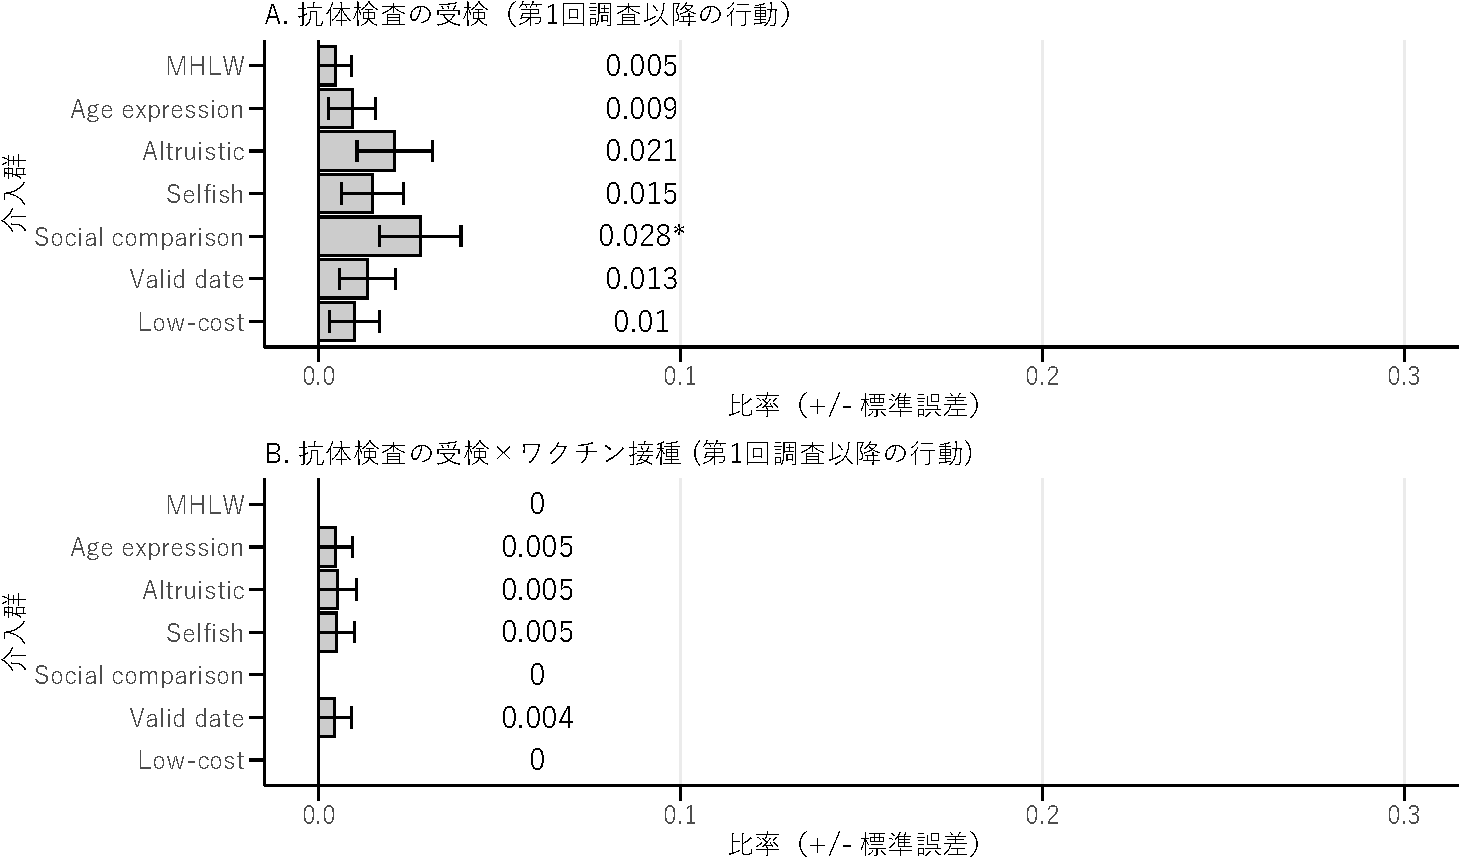
\includegraphics{C:/Users/vge00/Desktop/MHLW-Rubella-Project/2020-online-RCT/publish/body_files/figure-latex/show-act-coupon0-ttest-1} \caption{2019年度クーポン券配布対象外の男性に限定した行動に対するナッジ・メッセージの効果。データソース:Wave 2セレクションデータ。注)図中の数値は各群の比率を示す。星印は厚労省メッセージ群との平均値の差のt検定の結果であり、次の規則に従う:* p < 0.1、** p < 0.05、*** p < 0.01。}\label{fig:show-act-coupon0-ttest}
\end{figure}

図\ref{fig:show-act-coupon0-ttest}は各介入群の第1回調査以降の抗体検査受検比率と
第1回調査以降のワクチン接種比率である。
社会比較メッセージが厚労省メッセージよりも第1回調査以降の抗体検査の受検を促進しているが、
抗体検査とワクチン接種の両方を促進していない。
厚労省メッセージを読んだ人の約0.5\%が第1回調査以降に抗体検査を受検したが、
誰もワクチン接種をしていない。
また、社会比較メッセージを読んだ人の約2.8\%が第1回調査以降に抗体検査を受検したが、
誰もワクチン接種をしていない。
よって、社会比較メッセージの抗体検査受検に対する効果は約2.3\%ポイントであり、
これは統計的に10\%水準で有意である。
しかしながら、抗体検査とワクチン接種の両方に対する効果はゼロである。

ここまでの結果は表\ref{tab:show-covlist}で示した個人の観察可能な特徴をコントロールしても変化しない。
補論\ref{addtab}の表\ref{tab:show-int-coupon0-reg}と表\ref{tab:show-act-coupon0-reg}
はナッジ・メッセージの線形確率モデルの推定結果である。
奇数列はナッジ・メッセージのダミー変数のみを説明変数に加えているので、
これらの結果は二群間のt検定の結果
(図\ref{fig:show-int-coupon0-ttest}と図\ref{fig:show-act-coupon0-ttest})に対応している。
偶数列はナッジ・メッセージのダミー変数に加えて、表\ref{tab:show-covlist}の変数を説明変数に加えている。
列(4)は、これまでの結果に加えて、
年齢表現メッセージが抗体検査の受検に負の効果を持っていることを示しており、
これは統計的に5\%水準で有意である。

\begin{table}

\caption{\label{tab:show-tester-coupon0}2019年度クーポン券配布対象外の抗体検査受検者の動き}
\centering
\begin{threeparttable}
\begin{tabular}[t]{lcccc}
\toprule
\multicolumn{1}{c}{ } & \multicolumn{2}{c}{Negative antibody} & \multicolumn{2}{c}{Vaccination} \\
\cmidrule(l{3pt}r{3pt}){2-3} \cmidrule(l{3pt}r{3pt}){4-5}
Treatments & No & Yes & No  & Yes \\
\midrule
厚労省 & 1 & 0 & 1 & 0\\
年齢表現 & 0 & 2 & 1 & 1\\
利他強調 & 3 & 1 & 3 & 1\\
利己強調 & 2 & 1 & 2 & 1\\
社会比較 & 5 & 1 & 6 & 0\\
有効期限 & 2 & 1 & 2 & 1\\
低コスト & 2 & 0 & 2 & 0\\
\bottomrule
\end{tabular}
\begin{tablenotes}
\item Note: Fisher exact test (Outcome: Negative antibody): p = 0.466. Fisher exact test (Outcome: Vaccination): p = 0.568.
\end{tablenotes}
\end{threeparttable}
\end{table}

第\ref{coupon1}節で示したように、
ワクチン接種比率が抗体検査の受検比率より低い原因は、
抗体検査の陰性比率が低いことにある。
表\ref{tab:show-tester-coupon0}に抗体検査受検者の動きを示した。
各群の抗体検査の陰性比率は0\%から100\%の範囲にある。
とくに、厚労省メッセージの抗体検査の陰性比率は0\%(\(=0/1\))である。
抗体検査を促進した社会比較メッセージの陰性比率は17\%(\(=1/6\))である。
しかしながら、フィッシャーの正確検定より、
これらの二群の陰性比率の差は統計的に有意でない
(第6列より、p値は1)。

また、第\ref{coupon1}節と同様に、
抗体検査の結果が陰性である人のほとんどがワクチンを接種していることも明らかになった。
厚労省メッセージ群と低コストメッセージ群では、陰性者がいない。
残った介入群のうち、社会比較メッセージ群を除くすべての群において、
抗体検査の結果が陰性である人は全員ワクチンを接種していた。

\hypertarget{conclusion}{%
\section{議論と結論}\label{conclusion}}

本研究は、オンラインサーベイによるランダム化比較試験(RCT)を用いて、
風しんワクチンの接種を促進するためにどのようなナッジ・メッセージが有効であるかを明らかにした。
主な結果は以下の三つにまとめられる。
第一に、2019年度にクーポン券送付対象の年齢の男性のみに利他強調メッセージが抗体検査の受検を7.5\%ポイント促進した。
このメッセージの効果を金銭的価値で評価すると、一人当たりの金銭的価値は約2000円(約18ドル)であり、
その総額は約100億円(約9,700万ドル)である。
この効果は個人の観察可能な特徴に対して頑健であり、
サンプルサイズが小さいことを考慮したフィッシャーの正確検定でも、
この効果は5\%水準で有意である(表\ref{tab:show-tester-coupon1}の第4列)。
また、利己強調メッセージや社会比較メッセージの抗体検査の受検比率は利他強調メッセージ群のそれと有意な差ではない。
この意味で、二つのメッセージも抗体検査の受検を促進した可能性がある。
しかしながら、抗体検査の受検比率の差は検出力を十分に保てるほどの大きさではないので、
サンプルサイズを増やした再検証が必要である。

第二に、介入群に関わらず、抗体検査の結果が陰性である人のほとんどはワクチンを接種していた。
これは、抗体保有率を高めるために、陰性である人のワクチン接種率を高めるような政策ではなく、
抗体検査の受検比率を高めるような政策の方が効率的であることを示唆している。
したがって、利他強調メッセージは抗体保有率を高めるためのナッジ・メッセージとして有効である。

第三に、2019年度にクーポン券がオンデマンドでしか送付されない年齢層の男性に対してナッジ・メッセージは機能しなかった。
考えられる可能性が二つある。
第一に、2019年度にクーポン券の送付対象ではない男性は厚生労働省の無料クーポン券制度を認知していないという点である。
第1回調査の調査票A(ナッジ・メッセージを示す前の調査)で、我々は厚生労働省のクーポン券制度の認知度を調査した。
その結果、2019年度にクーポン券の送付対象ではない年齢層の男性の約
77.5\%
が厚生労働省のクーポン券制度を知らなかった。
仮にナッジ・メッセージを読んで、風しんの抗体検査やワクチン接種を受ける必要性を理解したとしても、
クーポン券の存在を知らない人はそれらの予防行動を自費で受けないといけないと考えている。
ナッジ・メッセージは予防行動のコストを上回るほどその価値を高められなかったのかもしれない。
第二に、クーポン券制度を認知していて無料接種対象の年齢であったとしても、
2019年度にクーポン券の送付対象ではない年齢の男性は自治体にクーポン券を発行してもらうように依頼する必要があるという点である。
クーポン券制度を認知している男性が無料で抗体検査やワクチン接種を受けられることを知っていても、
クーポン券の発行の手続き自体にコストが伴う。
したがって、ナッジ・メッセージはクーポン券の発行の手続きのコストを上回るほどその価値を高められなかったのかもしれない。

分析結果について考慮すべき点が一つある。
ナッジ・メッセージの行動に対する効果を推定するとき、
我々はWave 2で前回のアンケート調査以前に抗体検査もしくはワクチン接種を受けたと回答した人を除いている。
しかしながら、この回答は想起バイアスを伴っている可能性がある。
もしそうならば、サンプルセレクションに想起バイアスが伴うので、
Wave 2でWave 1以前に抗体検査もしくはワクチン接種を受けたという人を除くべきではない。
したがって、想起バイアスを想定した分析では、Wave 1で過去に抗体検査もしくはワクチン接種を受けたと回答した人を除いたサブサンプルと、
抗体検査やワクチン接種を受けた時期に基づかないアウトカム変数を用いるべきである。
想起バイアスを想定した分析では、
効果・統計的な有意性・効果の金銭的価値は大きく異なるものの、
利他強調メッセージが抗体検査の受検を促進していることを確認している
(詳細な結果は補論Bに示した)。

最後に、新たなナッジ政策の方向性を議論しておく。
第一に、クーポン券を得ることで無料で抗体検査やワクチン接種を受けられること、
そして、その手続きの方法を分かりやすく伝えるようなナッジ・メッセージは有効かもしれない。
2019年度にクーポン券が配布されなかった男性に対して、
我々が開発したナッジ・メッセージは有効ではなかった。
先に述べたように、その原因はそもそもクーポン券制度の存在を知らなかった、
もしくはクーポン券の発行の手続きのコストが高いことにあると考えられる。
こうした問題点を解消するようなナッジ政策は有効だろう。
ただし、これは今回の厚生労働省の風しん対策特有の問題であることに注意したい。
第二に、実際は抗体を保有していないが、風しんに感染した経験があると思っていたり、ワクチンを接種したと思っていて、
抗体を保有していると誤って信じているような人の抗体検査の受検を促進することである。
抗体保有の誤った信念を正すようなナッジ政策がより効率的に政策目標を達成できるだろう。
このようなナッジ政策の効果検証が今後の研究課題となる。

\newpage

\hypertarget{ux53c2ux8003ux6587ux732e}{%
\section*{参考文献}\label{ux53c2ux8003ux6587ux732e}}
\addcontentsline{toc}{section}{参考文献}

\hypertarget{refs}{}
\begin{CSLReferences}{1}{0}
\leavevmode\vadjust pre{\hypertarget{ref-Kinoshita2016}{}}%
Kinoshita, R., Nishiura, H., 2016. Assessing herd immunity against rubella in {Japan}: A retrospective seroepidemiological analysis of age-dependent transmission dynamics. BMJ Open 6, e009928. doi:\href{https://doi.org/10.1136/bmjopen-2015-009928}{10.1136/bmjopen-2015-009928}

\leavevmode\vadjust pre{\hypertarget{ref-Nishiura2015}{}}%
Nishiura, H., Kinoshita, R., Miyamatsu, Y., Mizumoto, K., 2015. Investigating the immunizing effect of the rubella epidemic in {Japan}, 2012-14. International Journal of Infectious Diseases 38, 16--18. doi:\href{https://doi.org/10.1016/j.ijid.2015.07.006}{10.1016/j.ijid.2015.07.006}

\leavevmode\vadjust pre{\hypertarget{ref-Plans-Rubio2012}{}}%
Plans-Rubió, P., 2012. Evaluation of the establishment of herd immunity in the population by means of serological surveys and vaccination coverage. Human Vaccines \& Immunotherapeutics 8, 184--188. doi:\href{https://doi.org/10.4161/hv.18444}{10.4161/hv.18444}

\end{CSLReferences}

\end{document}
